%%%%%%%%%%%%%%%%%%%%%%%%%%%%%%%%%%%%%%%%%%
%%%%%%%%%%%%%                 %%%%%%%%%%%%
%%%%%%%%%%%%%    EXERCISE 1   %%%%%%%%%%%%
%%%%%%%%%%%%%                 %%%%%%%%%%%%
%%%%%%%%%%%%%%%%%%%%%%%%%%%%%%%%%%%%%%%%%%
\begin{exercise}[]{(30 points) Ping 10.0.0.111 from 10.0.0.112 (in your terminal of VM2) and use Wireshark to monitor the interfaces s2 and enp0s8, and describe the protocols used in this procedure and your findings.}
  \begin{solution}
  \par{~}
  As has been shown in Figure \ref{fig:ex1-1}, we can ping 10.0.0.111 from 10.0.0.112. Figure \ref{fig:ex1-2} shows that interface s2 uses ICMP protocol for requesting and replying the ping command. For interface enp0s8, besides ICMP protocol, ARP protocol is also used in \ref{fig:ex1-3}.
  
  The Address Resolution Protocol (ARP) is a communication protocol used for discovering the link layer address, such as a MAC address, associated with a given internet layer address, typically an IPv4 address. Therefore s1 in our host can know how to reach s2 in the network.
  \begin{figure}[ht]
    \begin{center}
    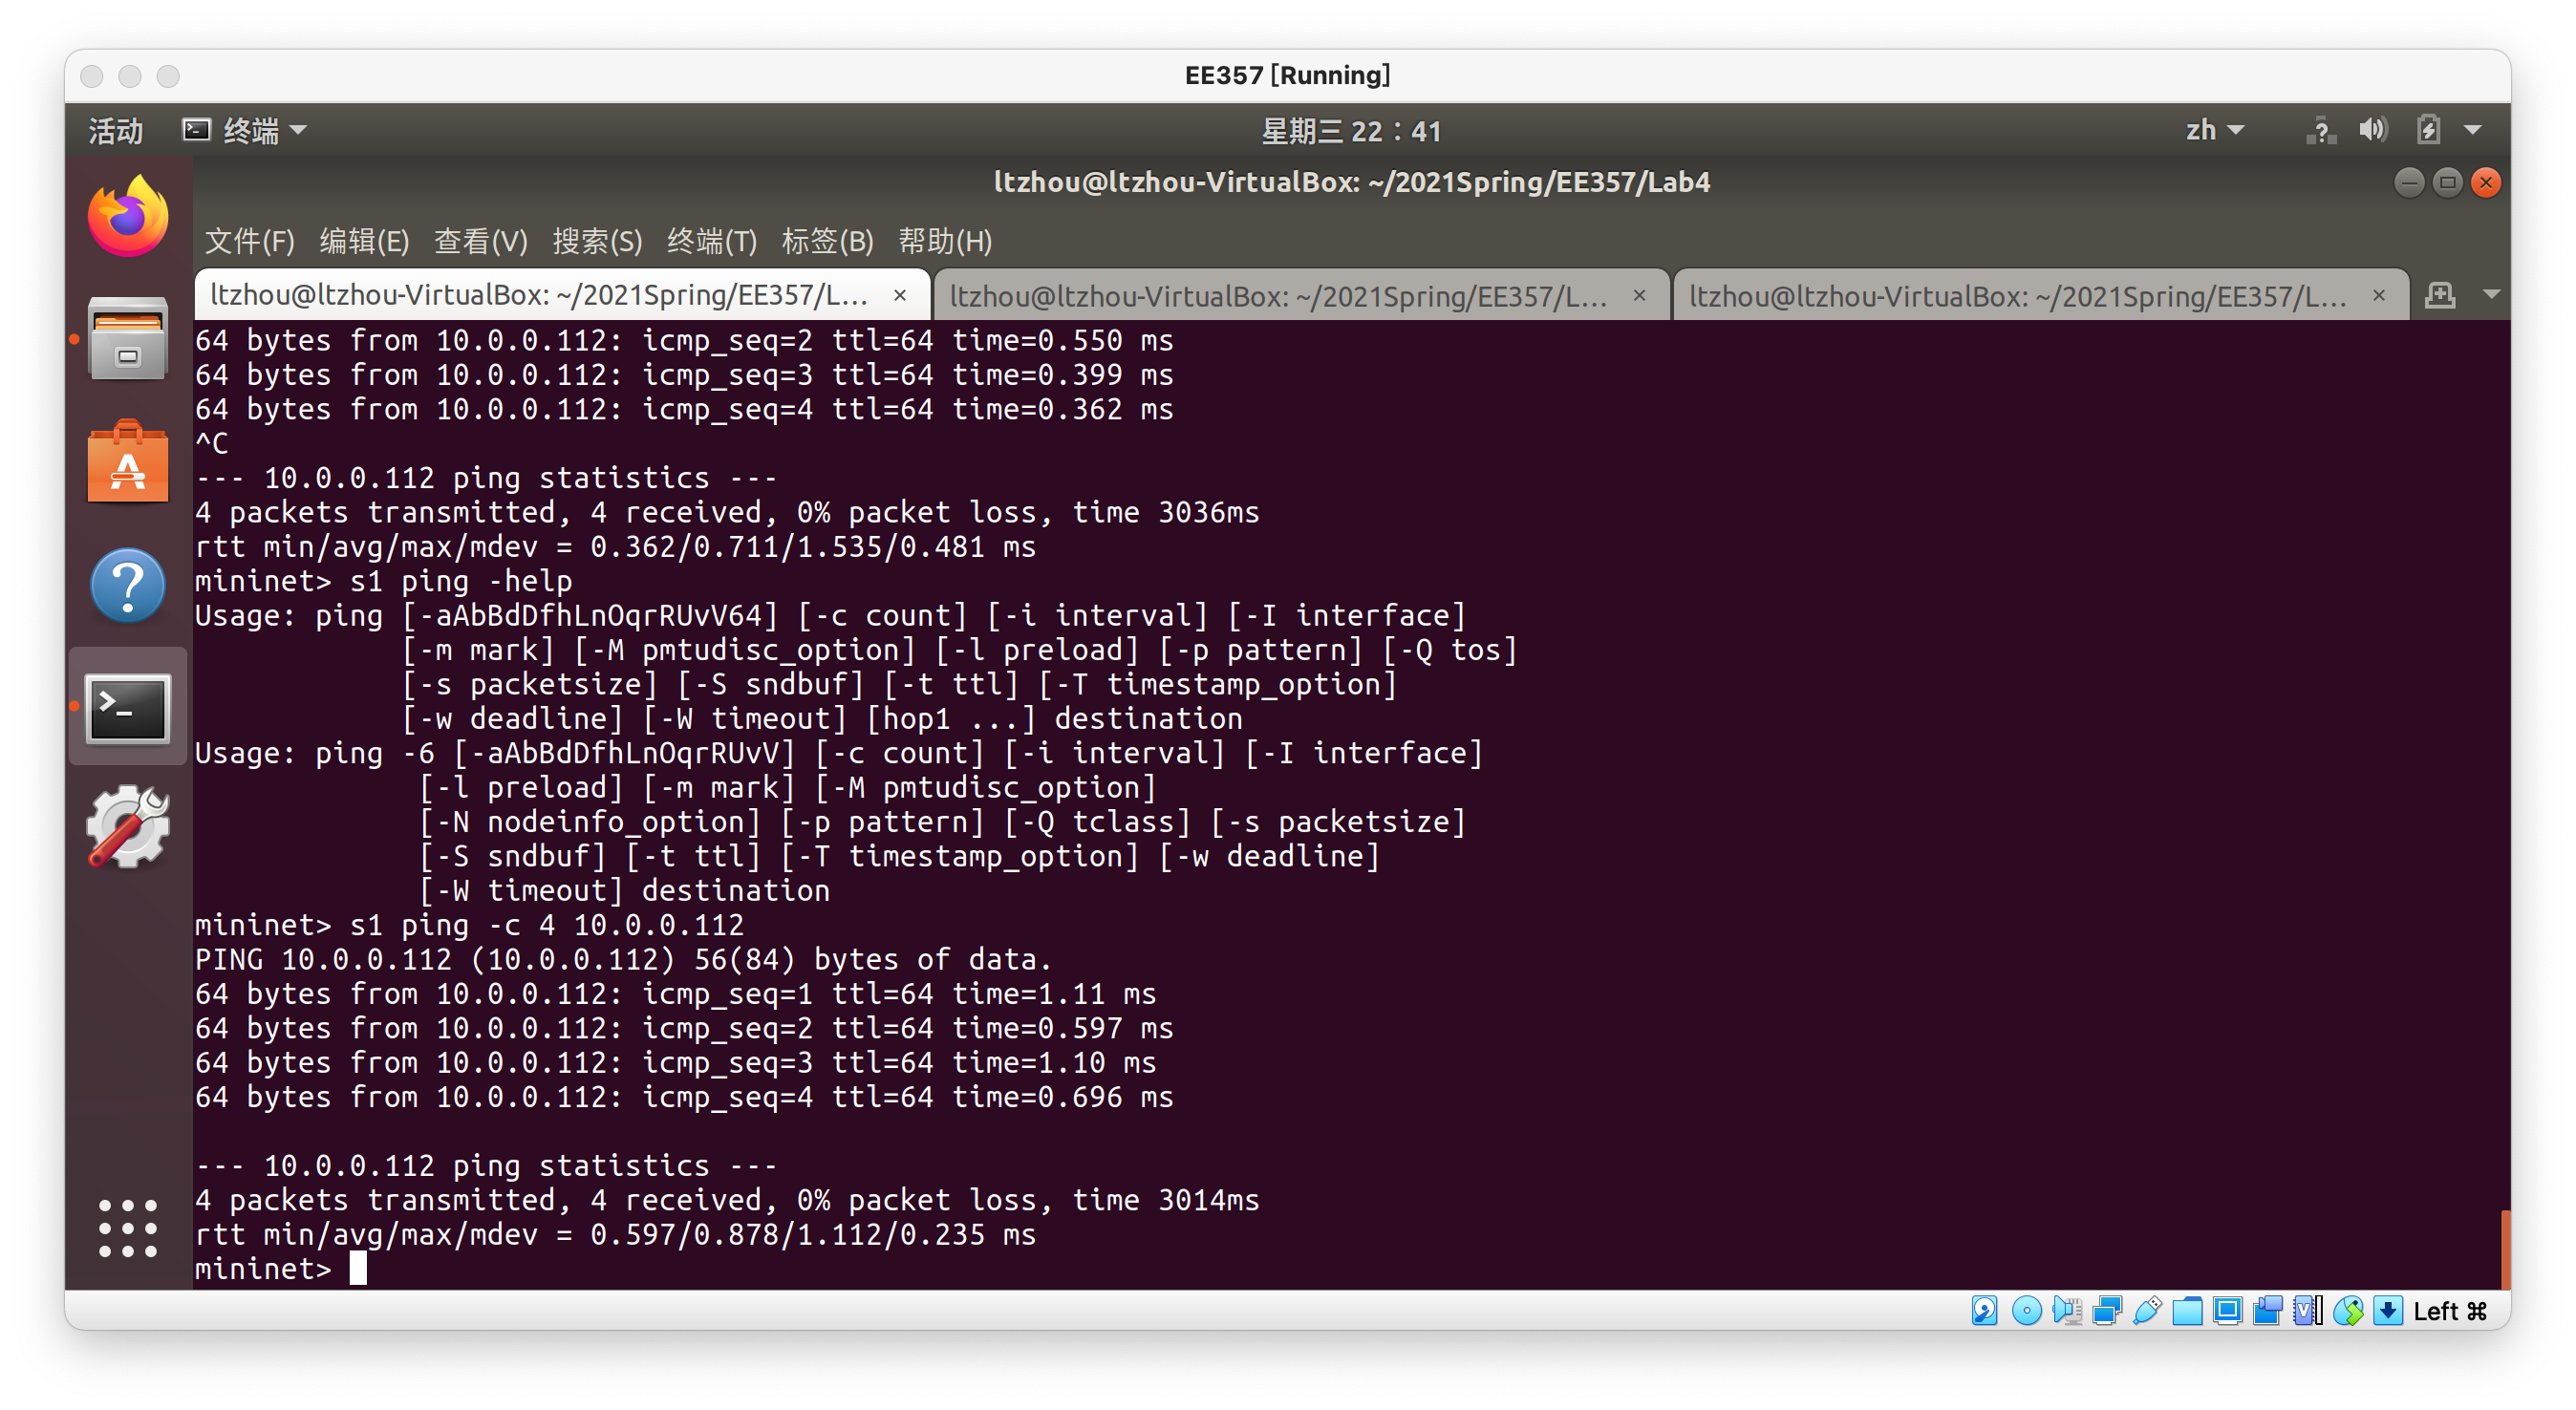
\includegraphics[width=12cm]{img/lab4/ex1-1.png}
    \caption{ping 10.0.0.112 from 10.0.0.111}
    \label{fig:ex1-1}
    \end{center}
  \end{figure}

  \begin{figure}[ht]
    \begin{center}
    \begin{minipage}[t]{0.48\linewidth}
        \centering
        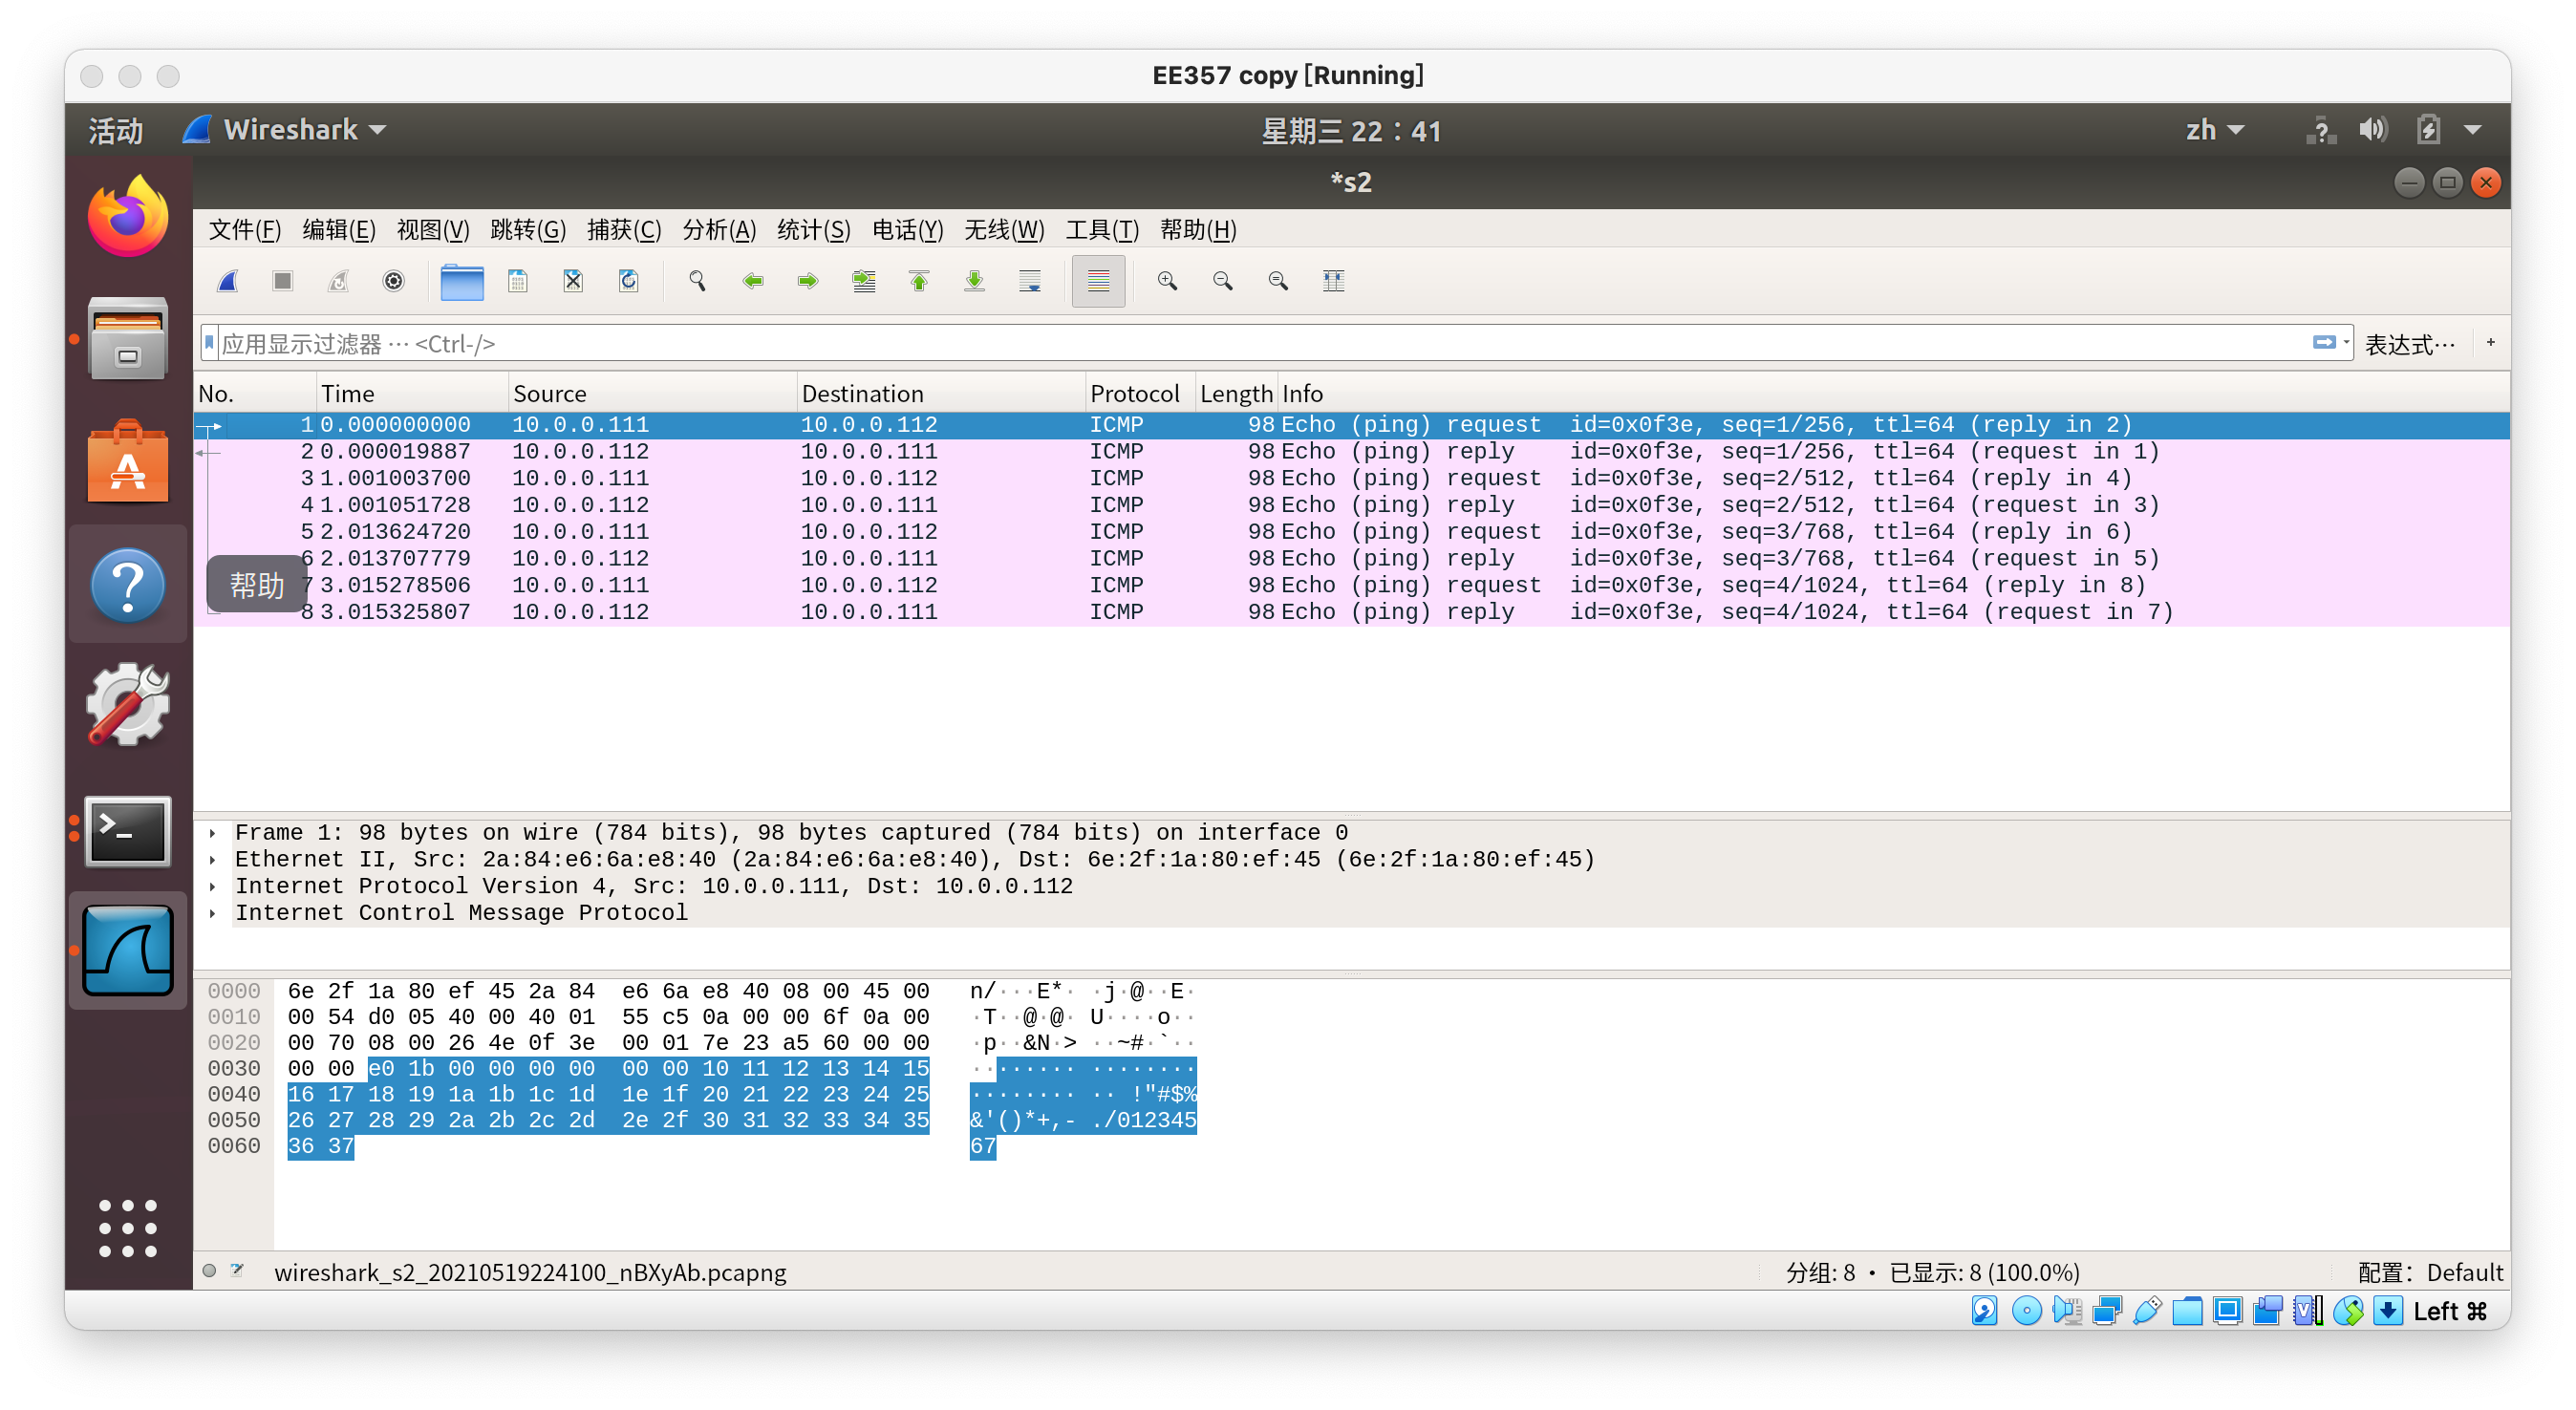
\includegraphics[width=1\linewidth]{img/lab4/ex1-2.png}
        \caption{Wireshark result of s2 interface}
        \label{fig:ex1-2}
    \end{minipage}
    \begin{minipage}[t]{0.48\linewidth}
        \centering
        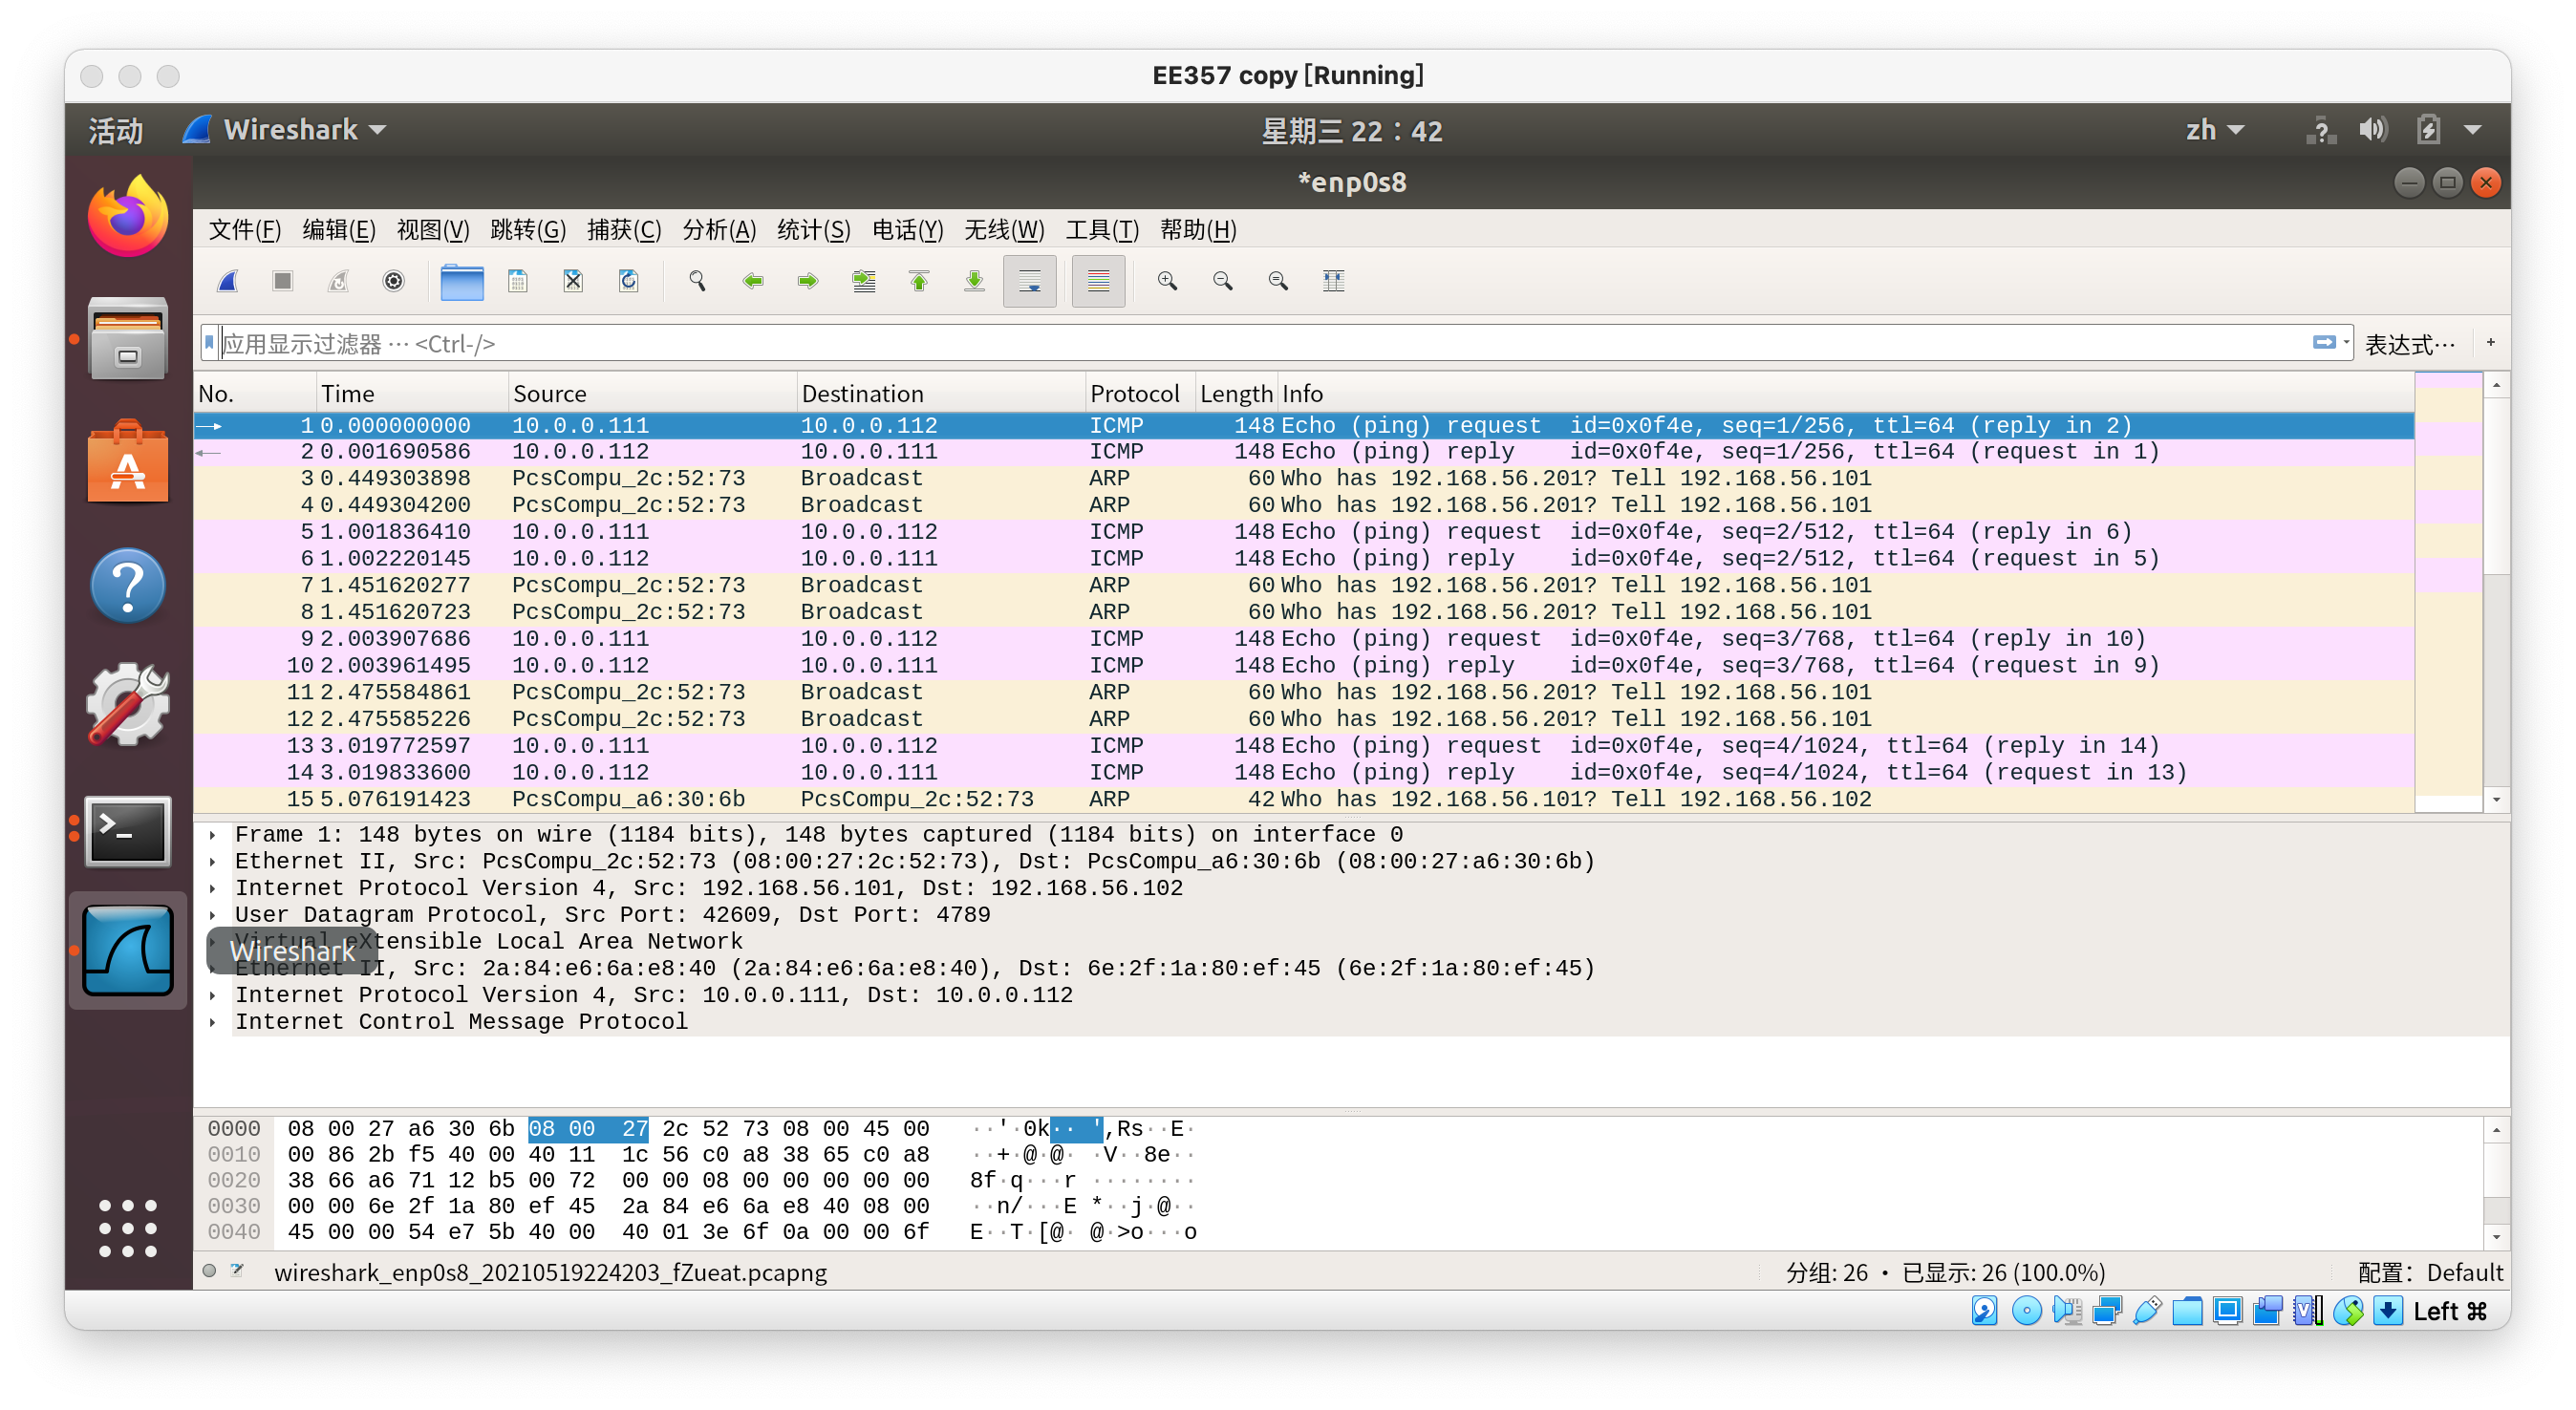
\includegraphics[width=1\linewidth]{img/lab4/ex1-3.png}
        \caption{Wireshark result of enp0s8 interface}
        \label{fig:ex1-3}
    \end{minipage}
    \end{center}
  \end{figure}

  \end{solution}
  \label{ex1}
\end{exercise}

\newpage

%%%%%%%%%%%%%%%%%%%%%%%%%%%%%%%%%%%%%%%%%%
%%%%%%%%%%%%%                 %%%%%%%%%%%%
%%%%%%%%%%%%%    EXERCISE 2   %%%%%%%%%%%%
%%%%%%%%%%%%%                 %%%%%%%%%%%%
%%%%%%%%%%%%%%%%%%%%%%%%%%%%%%%%%%%%%%%%%%
\begin{exercise}[]{(50 points) Use iperf to test the network bandwidth between the two virtual machines
    \begin{enumerate}
        \item Test the bandwidth between 192.168.56.101 and 192.168.56.102
        \item Test the bandwidth between 10.0.0.1/10.0.0.2/10.0.0.111 and 10.0.0.3
    \end{enumerate}
    Compare the above results and explain the reason. (Hint: you may need to specify a reasonable MTU size in order for your iperf to work in this case. Please also think about why.)}
  \begin{solution}
  \par{~}

  We first test the bandwidth between 192.168.56.101 and 192.168.56.102 directly on the virtual machine, which shows that the bandwidth is about 3.38 Gbits/sec in Figure \ref{fig:ex2-1-1}, \ref{fig:ex2-1-2}.

  Then we test the bandwidth between 10.0.0.1/10.0.0.2/10.0.0.111 and 10.0.0.3 using xterm in the MiniNet. However, the iperf fails in Figure \ref{fig:ex2-2-1}, \ref{fig:ex2-2-2}. This is because VXLAN adds 50 to 54 bytes of additional header information to the original Ethernet frame. We must increase the MTU of the underlying network. 
  
  In this case, configure the MTU of the physical interfaces that participate in the VXLAN network to be 2000 greater than the typical MTU of 1500, indicated in Figure \ref{fig:ex2-2-6}. After the configuration, the iperf command succeeds and the bandwidths between 10.0.0.3 and 10.0.0.1/10.0.0.2/10.0.0.111 are 918 Mbits/sec, 839 Mbits/sec, and 930 Mbits/sec respectively, in Figure \ref{fig:ex2-2-4}, \ref{fig:ex2-2-5}.

  \begin{figure}[ht]
    \begin{center}
    \begin{minipage}[t]{0.48\linewidth}
        \centering
        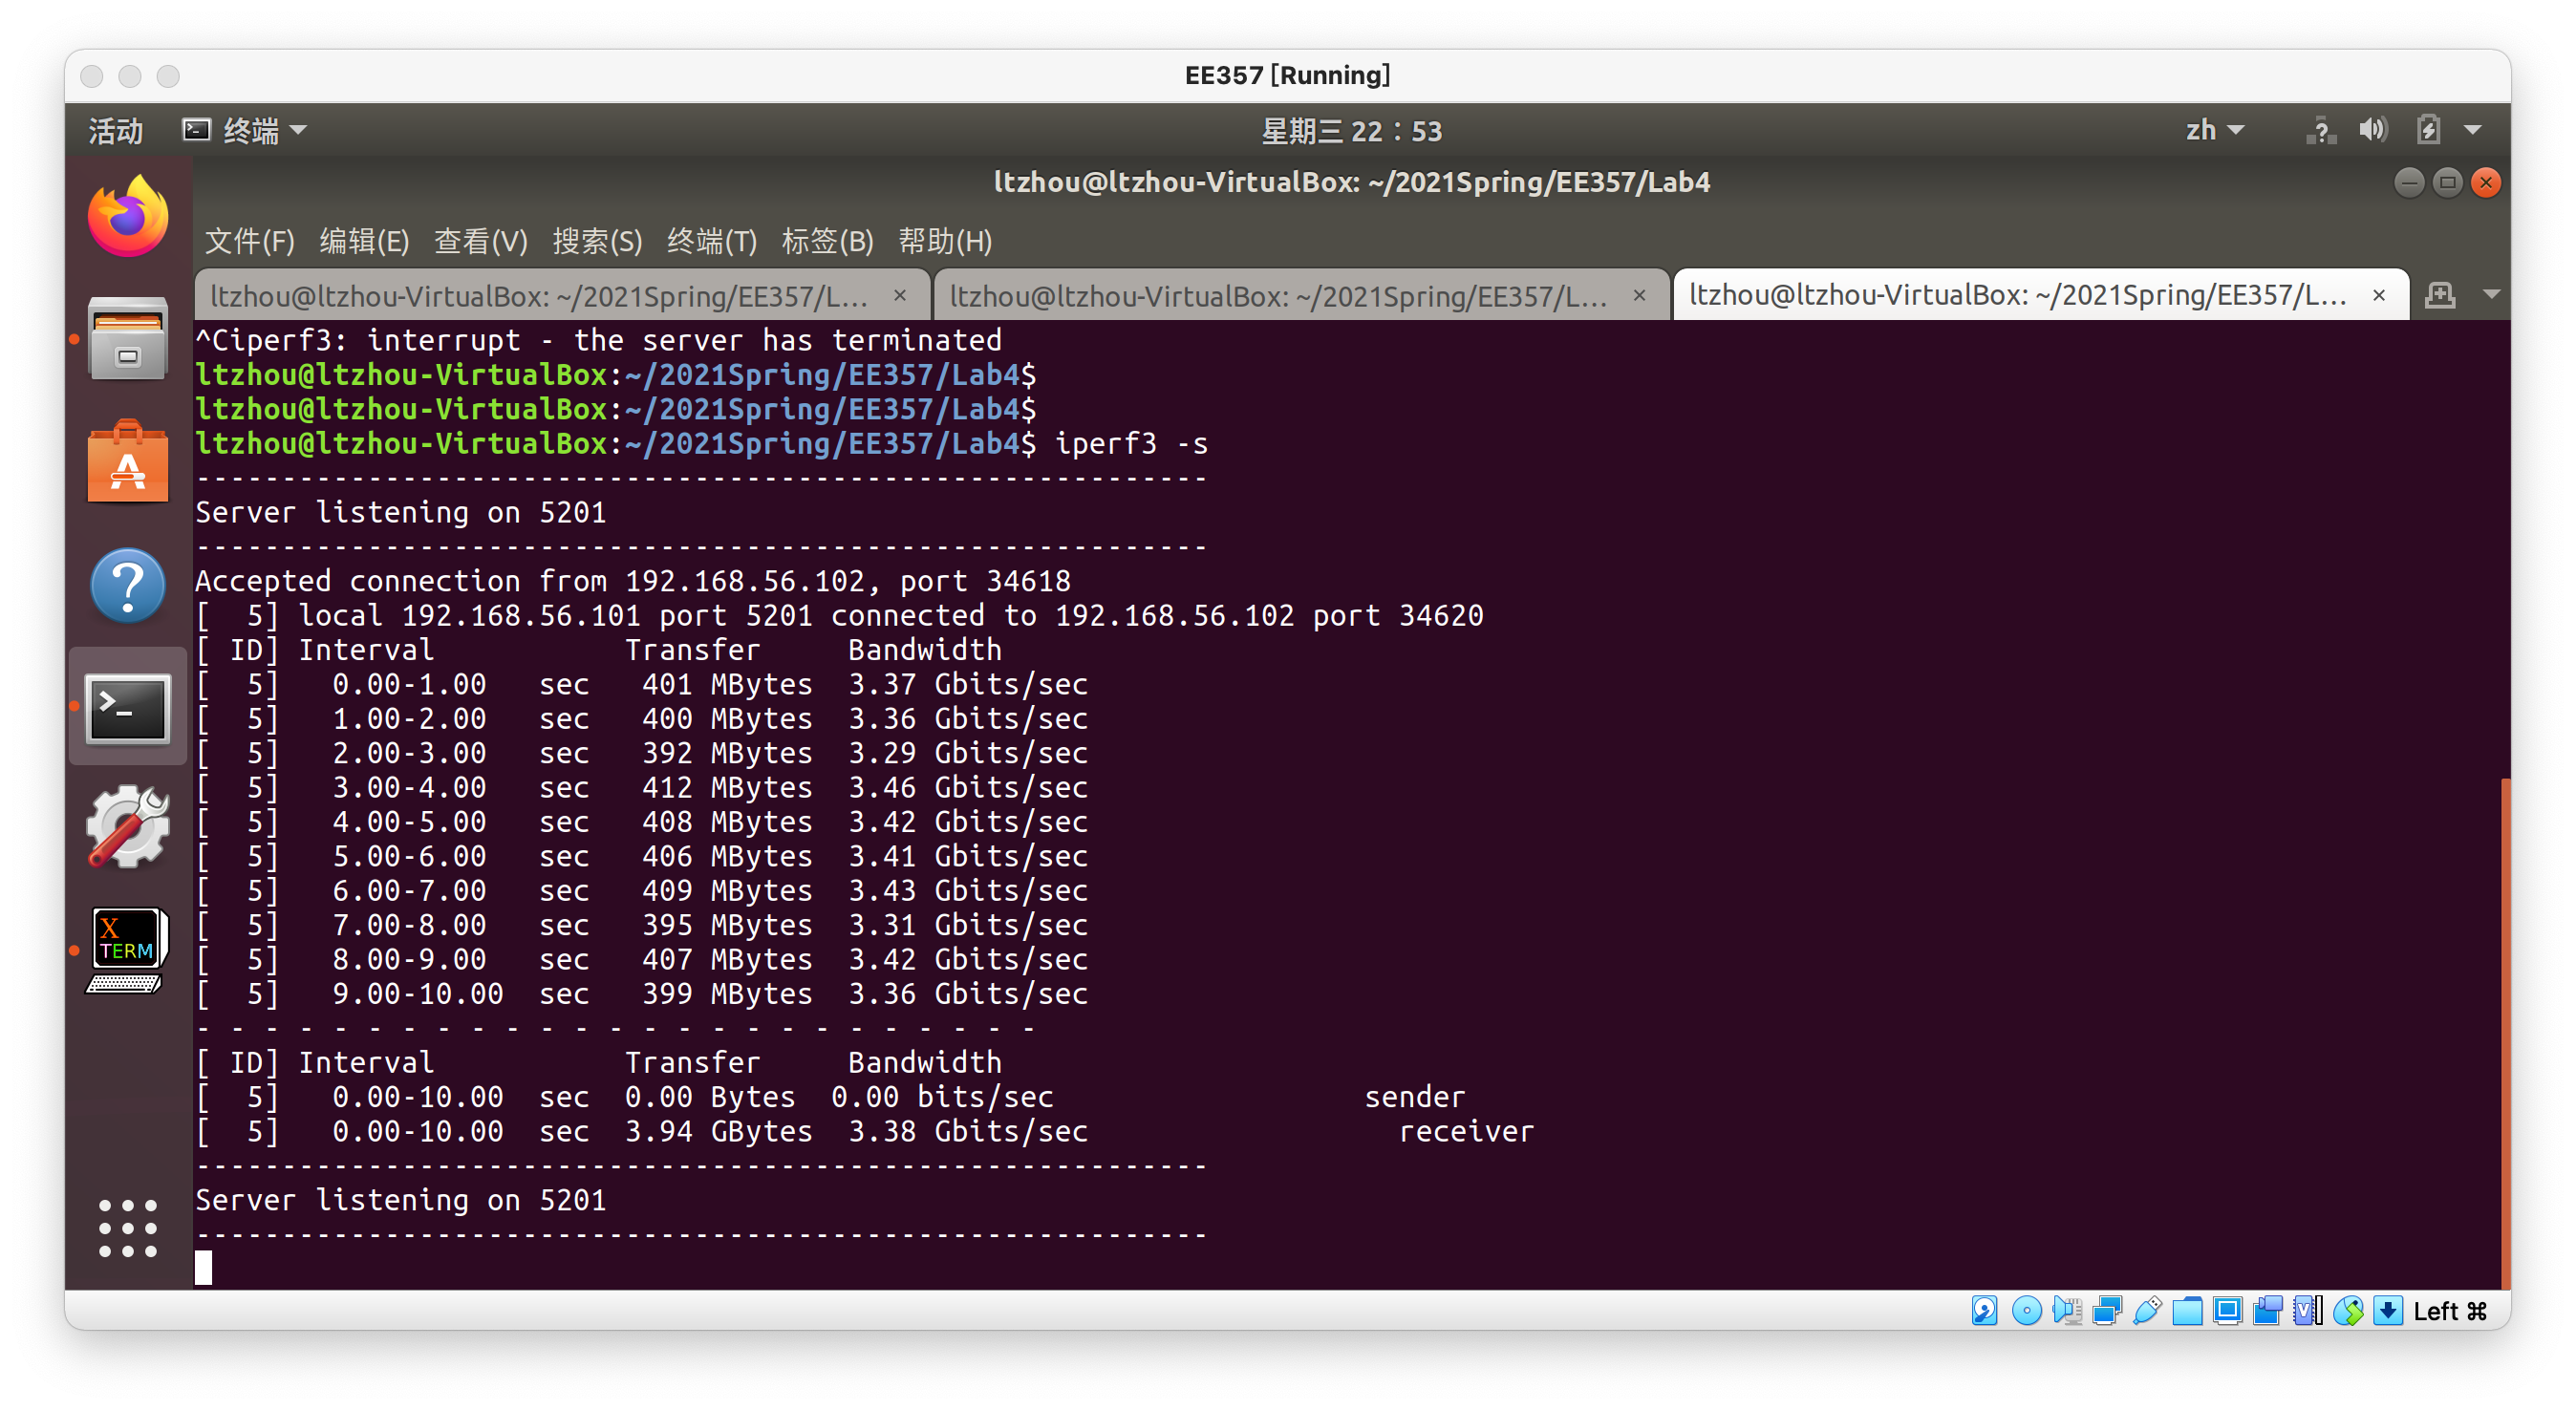
\includegraphics[width=1\linewidth]{img/lab4/ex2-1-1.png}
        \caption{iperf result of 192.168.56.101}
        \label{fig:ex2-1-1}
    \end{minipage}
    \begin{minipage}[t]{0.48\linewidth}
        \centering
        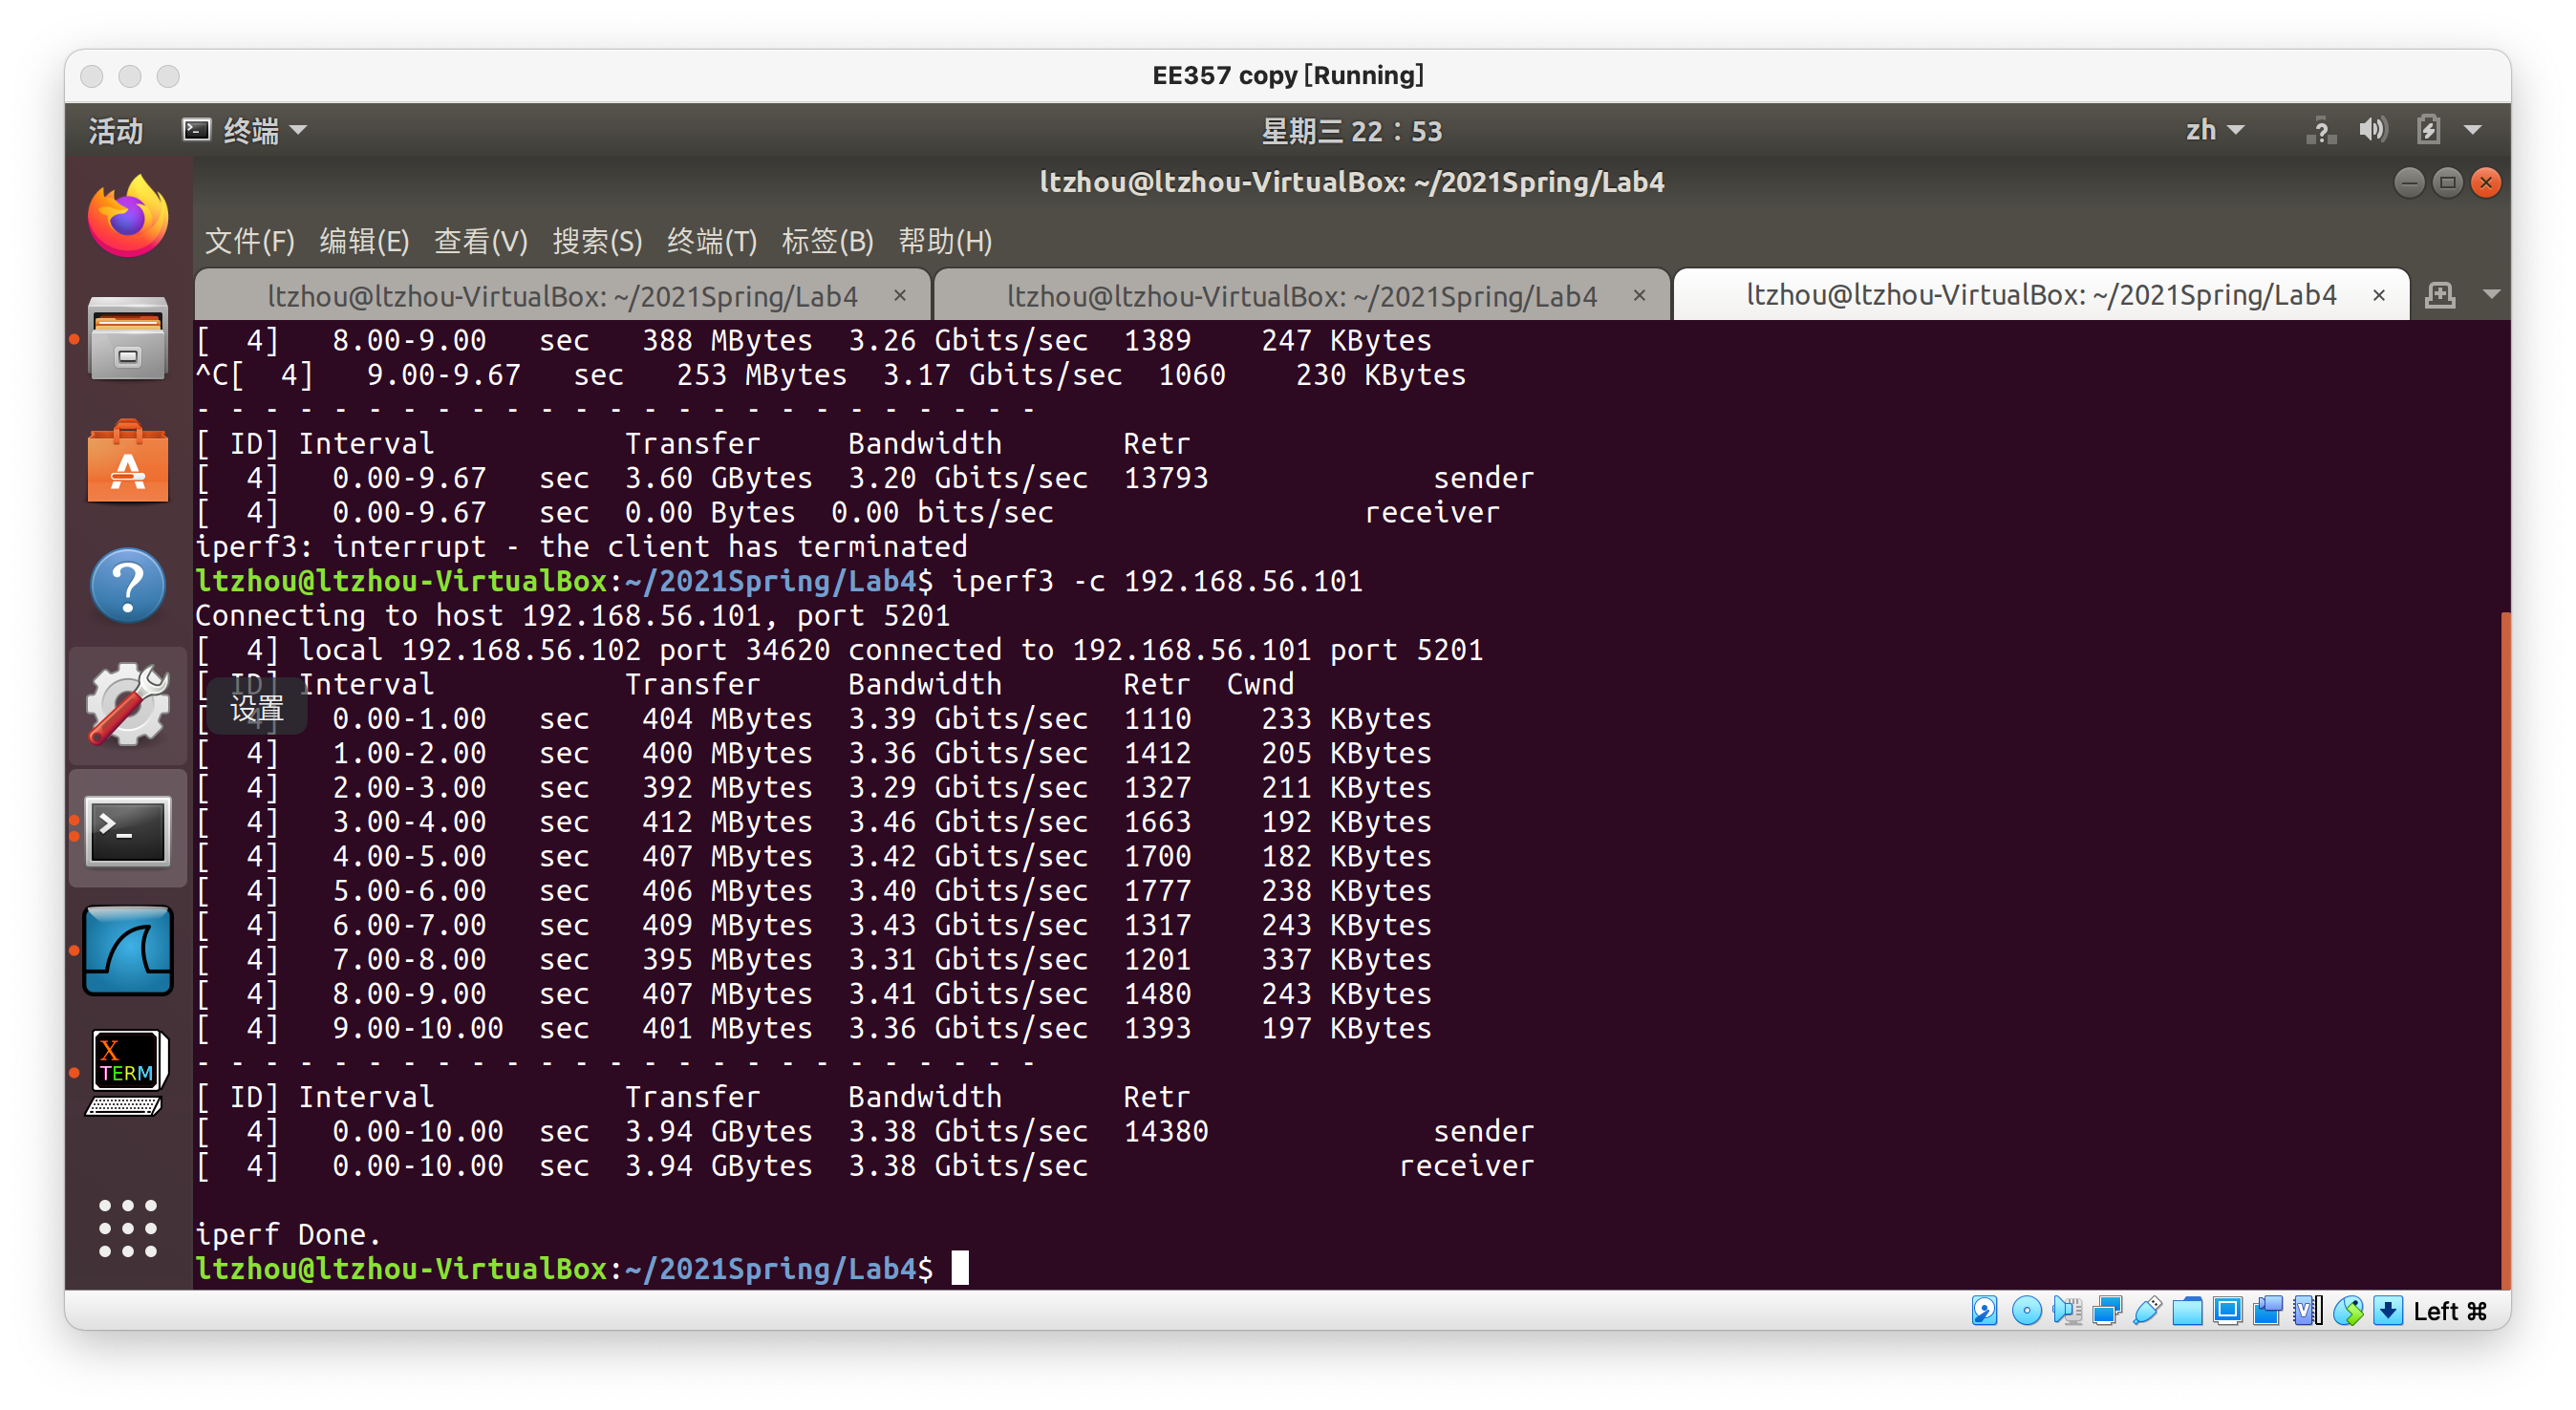
\includegraphics[width=1\linewidth]{img/lab4/ex2-1-2.png}
        \caption{iperf result of 192.168.56.102}
        \label{fig:ex2-1-2}
    \end{minipage}
    \end{center}
  \end{figure}

  \begin{figure}[ht]
    \begin{center}
    \begin{minipage}[t]{0.48\linewidth}
        \centering
        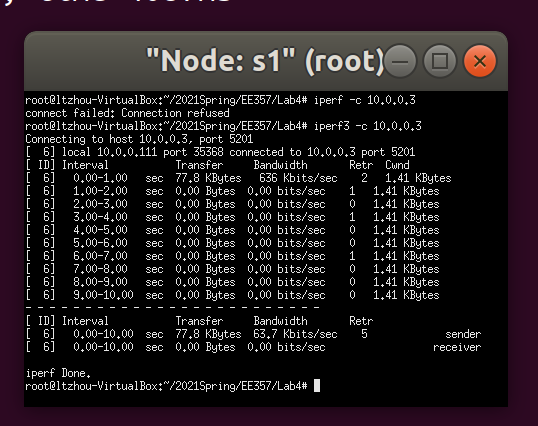
\includegraphics[width=0.7\linewidth]{img/lab4/ex2-2-1.png}
        \caption{Failure of iperf measurement for 10.0.0.111}
        \label{fig:ex2-2-1}
    \end{minipage}
    \begin{minipage}[t]{0.48\linewidth}
        \centering
        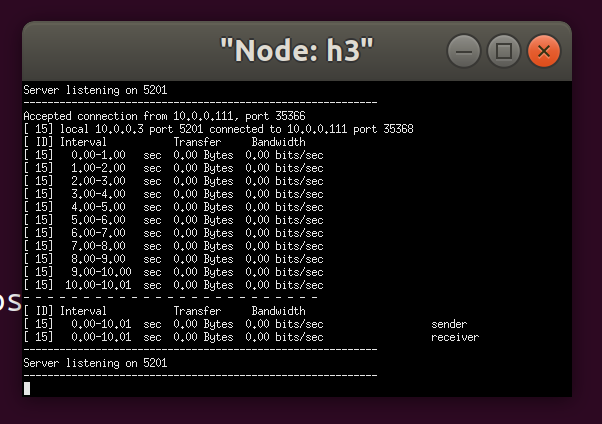
\includegraphics[width=0.7\linewidth]{img/lab4/ex2-2-2.png}
        \caption{Failure of iperf measurement for 10.0.0.3}
        \label{fig:ex2-2-2}
    \end{minipage}
    \end{center}
  \end{figure}

  \begin{figure}[ht]
    \begin{center}
    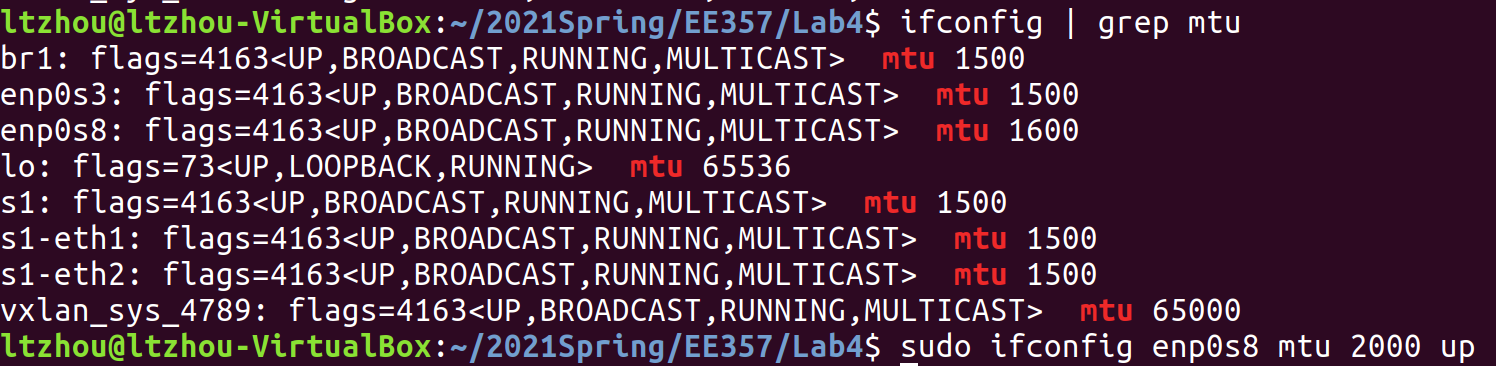
\includegraphics[width=12cm]{img/lab4/ex2-2-6.png}
    \caption{Change the MTU of the underlying physical interface}
    \label{fig:ex2-2-6}
    \end{center}
  \end{figure}

  \begin{figure}[ht]
    \begin{center}
    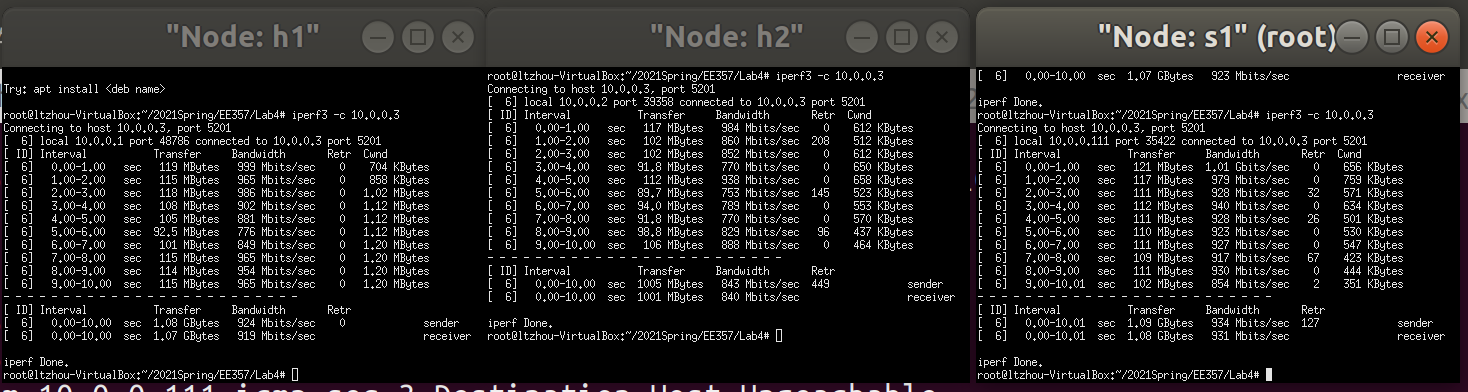
\includegraphics[width=16cm]{img/lab4/ex2-2-4.png}
    \caption{iperf measurement for 10.0.0.1, 10.0.0.2, 10.0.0.111 as clients}
    \label{fig:ex2-2-4}
    \end{center}
  \end{figure}

  \begin{figure}[ht]
    \begin{center}
    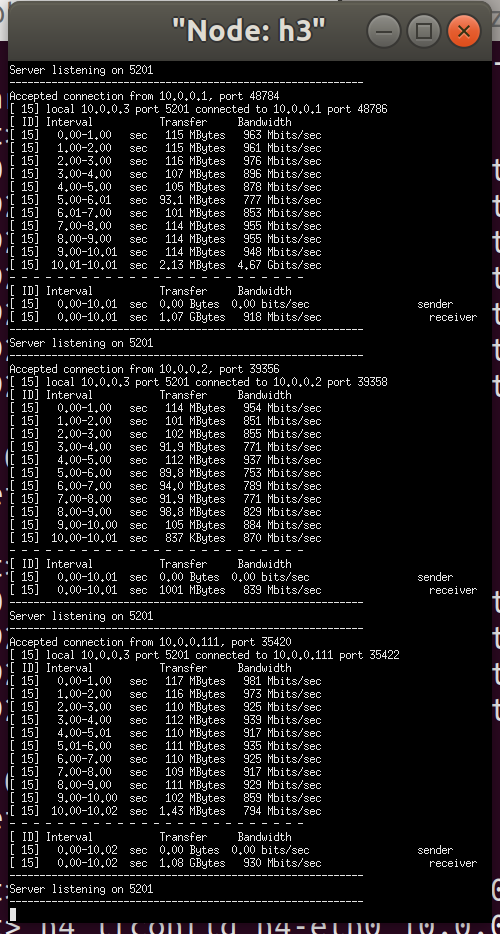
\includegraphics[width=6cm]{img/lab4/ex2-2-5.png}
    \caption{iperf measurement for 10.0.0.3 as server}
    \label{fig:ex2-2-5}
    \end{center}
  \end{figure}

  \end{solution}
  \label{ex2}
\end{exercise}

\newpage

%%%%%%%%%%%%%%%%%%%%%%%%%%%%%%%%%%%%%%%%%%
%%%%%%%%%%%%%                 %%%%%%%%%%%%
%%%%%%%%%%%%%    EXERCISE 3   %%%%%%%%%%%%
%%%%%%%%%%%%%                 %%%%%%%%%%%%
%%%%%%%%%%%%%%%%%%%%%%%%%%%%%%%%%%%%%%%%%%
\begin{exercise}[]{(20 points) Similar to Q2, use ping to test the network latency and analyze your results.}
  \begin{solution}
  \par{~}

  The latency between 192.168.56.101 and 192.168.56.102 is 0.836ms on average, shown in Figure \ref{fig:ex3-1}.

  The latency between 10.0.0.3 and 10.0.0.1/10.0.0.2/10.0.0.111 is 0.905ms, 2.054ms, and 1.941ms on average respectively, shown in Figure \ref{fig:ex3-2}. Note that receiving the first ping reply usually takes a much longer time than others.

    \begin{figure}[ht]
    \begin{center}
    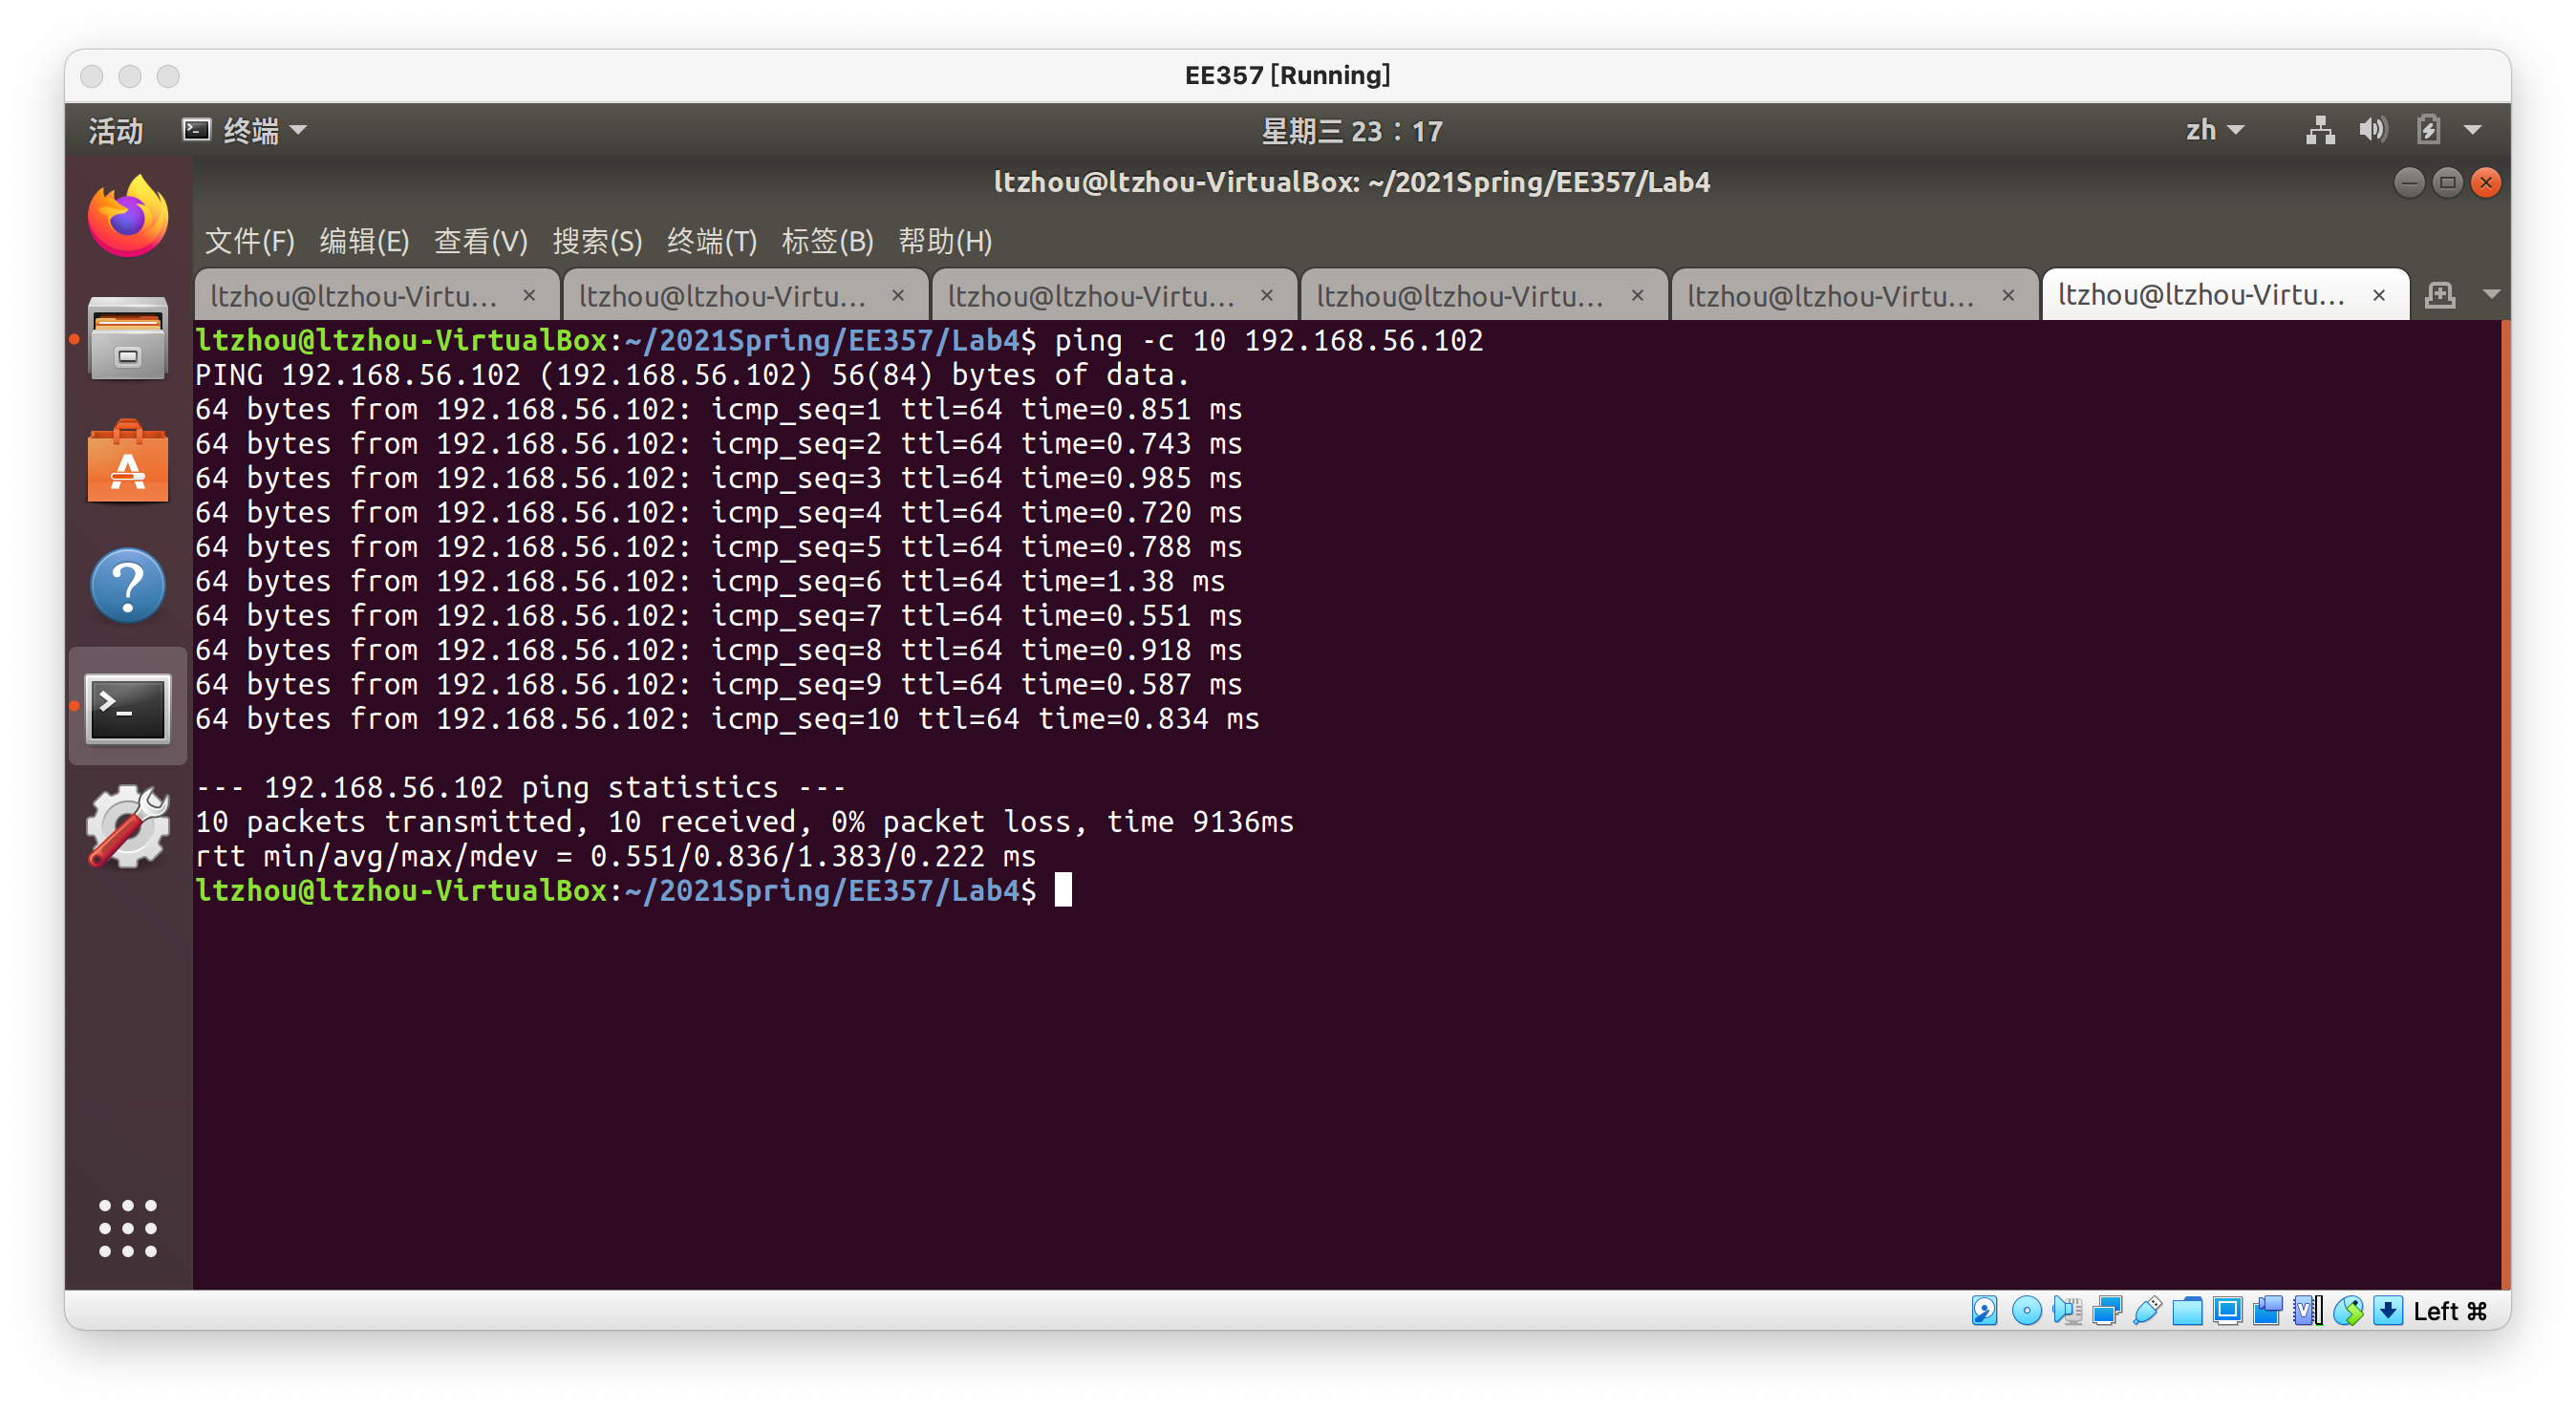
\includegraphics[width=12cm]{img/lab4/ex3-1}
    \caption{Ping latency between 192.168.56.101 and 192.168.56.102}
    \label{fig:ex3-1}
    \end{center}
    \end{figure}


    \begin{figure}[ht]
        \begin{center}
        \begin{minipage}[t]{0.3\linewidth}
            \centering
            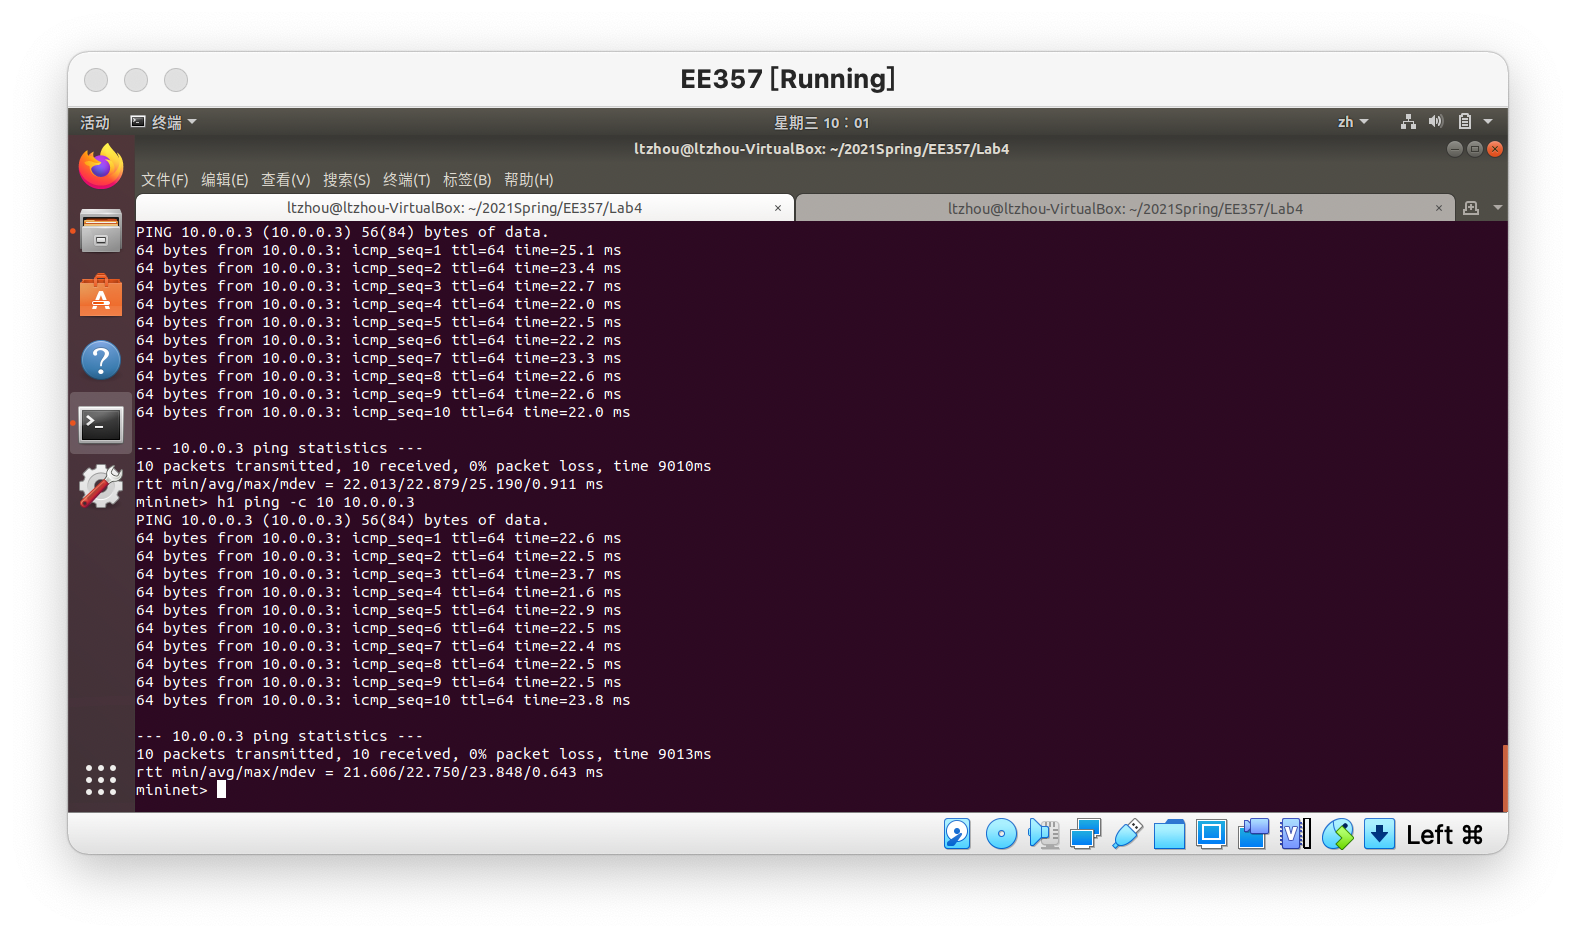
\includegraphics[width=0.9\linewidth]{img/lab4/ex3-2.png}
        \end{minipage}
        \begin{minipage}[t]{0.3\linewidth}
            \centering
            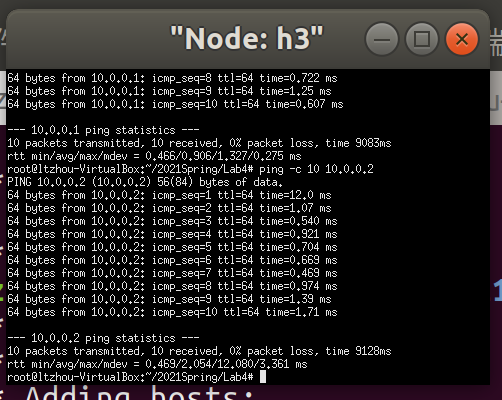
\includegraphics[width=0.9\linewidth]{img/lab4/ex3-3.png}
        \end{minipage}
        \begin{minipage}[t]{0.3\linewidth}
            \centering
            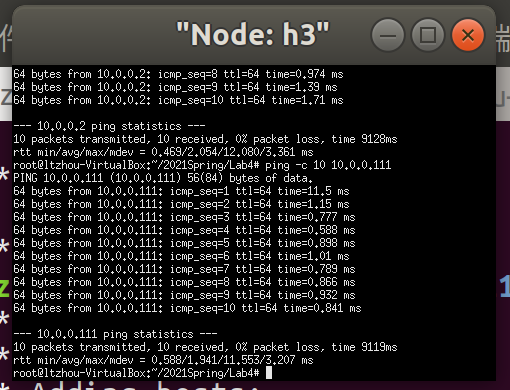
\includegraphics[width=0.9\linewidth]{img/lab4/ex3-4.png}
        \end{minipage}
        \caption{Ping latency from 10.0.0.3 to 10.0.0.1/10.0.0.2/10.0.0.111
        \label{fig:ex3-2}}
        \end{center}
    \end{figure}
  \end{solution}
  \label{ex3}
\end{exercise}